\section{Communication chain}
The communication chain is the set of elements that transforms data into a transmittable waveform. It consists of data pre-processors, modulation units and several recovery units for time, phase and frequency synchronization. An overview of the implemented communication chain is given in \reff{commchain_overview}

\begin{figure}[H]
    \centering
    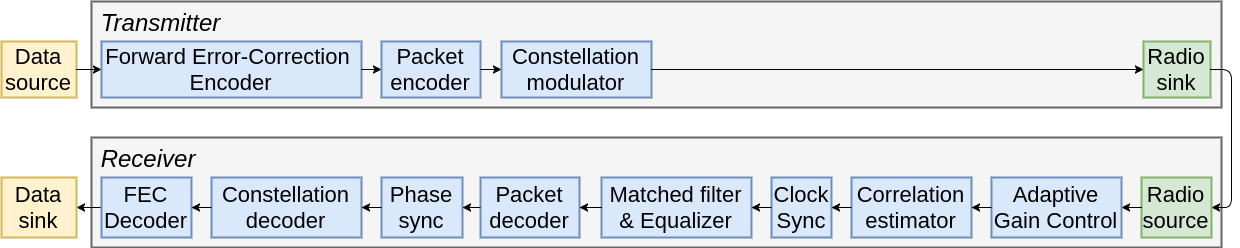
\includegraphics[width=1\textwidth]{img_commchain/overview.png}
    \caption{Communication chain overview}
    \label{fig:commchain_overview}
\end{figure}



\subsection{Pulse shaping}

The implemented packet encoder outputs constellation symbols. These symbols are processed by an upsampler and pulse shaper, in order to limit the bandwidth when transmitting. A common filter is a root raised cosine. At the receiver side, the signal can be convoluted with the matched filter so that the transmission is free of intersymbol interference. The spectrum of a transmissed stream, shaped with a root raised cosine filter, is shown in \reff{channel_spectrum}.

\begin{figure}[H]
    \centering
    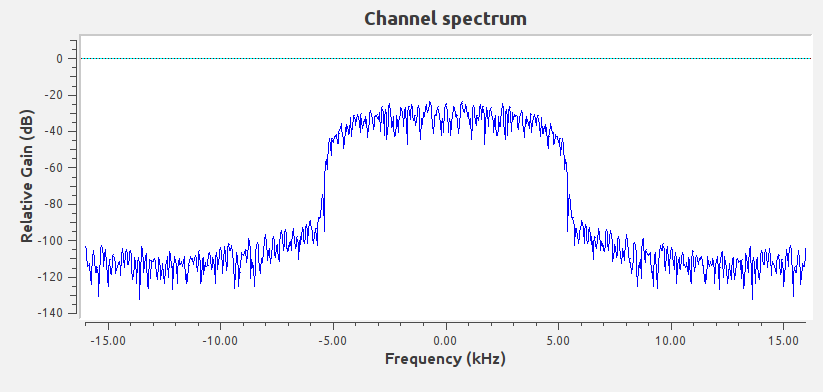
\includegraphics[width=0.8\textwidth]{img_commchain/channel_spectrum.png}
    \caption{Channel spectrum at baseband, RRC-filter with roll-off factor 0.35 and stop-band attenuation of 100 dB}
    \label{fig:channel_spectrum}
\end{figure}




\subsection{Frame synchronization}
The frame synchronization unit detects the start of packets. A common way is to prepend a preamble or access code sequence to the packet content so the receiver side can look for the preamble. After correlating the stream at the receiver with a modulated reference preamble, the packet start can be indicated by detecting correlation peaks.
\subsubsection{GNU Radio situation}
A large number of blocks for synchronization are included in the default GNU Radio installation. The most notable blocks are the \textit{Correlation Estimator}, \textit{Correlate Access Code} and \textit{Correlate and Sync}, where the latter is deprecated since GNU Radio 3.7.10. \medskip


The Correlation Estimator block is the most advanced and updated implementation. The block correlates a given modulated preamble with the incoming stream, and indicates correlation peaks with a tag called \textit{"corr\_est"}. \medskip

The block has a parameter \textit{Tag marking delay} which is used to shift the tag position compared to the incoming data stream. This shifting functionality is required because of two reasons. The first reason is that the convolution, used to pulse shape the reference preamble, introduces extra samples at the beginning and end of the preamble sequence because of the edge effect. When calculating the correlation with the incoming data stream, the tag will be placed at a fixed offset of the real position. The second reason is that some blocks in the communication chain do not preserve the correct tags positions, compared to the samples. The tag delay parameter should be set manually by looking at the output scopes.\medskip

\begin{figure}[H]
    \centering
    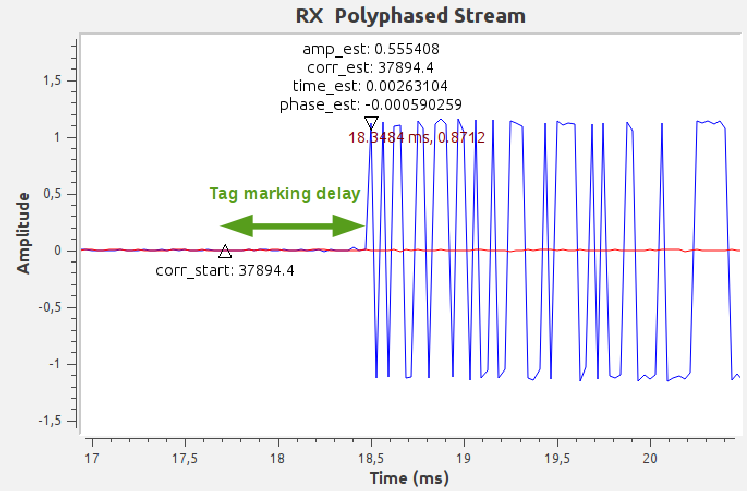
\includegraphics[width=0.8\textwidth]{img_commchain/tag_marking_delay2.png}
    \caption{The \textit{corr\_start} tag indicates where the Correlation Estimator block detected the preamble. The other tags are shifted by the number of samples that is given in the Tag Marking Delay field.}
    \label{fig:tag_marking_delay2}
\end{figure}

The $gr$-$digital$ package includes several synchronization examples, which are unfortunately broken in GNU Radio 3.7.9 and 3.7.10. The \textit{test\_corr\_est.grc} example has a threshold that is far too small, which causes a large amount of false-positives. In addition, the "Tag marking delay" is wrong. Many GNU Radio users have reported these issues \cite{corr_est_github_issue}.





\subsubsection{Pulse shaping the reference preamble}
The Correlation Estimator block expects a modulated and shaped preamble as input argument. \medskip

GNU Radio has a complementary block to modulate and pulse shape a byte stream, called Modulate Vector. In this project however, the preamble is defined as a pre-mapped sequence of complex symbols. To pulse shape the mapped vector, a new block was implemented in Python. The block is called Pulse Shape Vector and will pulse shape a given vector with a given filter. \medskip

\begin{figure}[H]
    \centering
    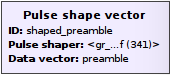
\includegraphics[width=0.25\textwidth]{img_commchain/pulseshaper_block.png}
    \caption{Pulse Shape Vector block in GNU Radio Companion}
    \label{fig:pulseshaper_block}
\end{figure}

The block accepts three parameters: 
\begin{tight_itemize}
\item ID: the variable name for the shaped preamble (output of the block)
\item Data vector: the variable name of the mapped preamble
\item Pulse shaper: definition of a filter in GNU Radio.
When using a polyphase filterbank with root raised cosine taps, the filter is defined is as follows:
\begin{minted}[frame=single,breaklines=true]{C}
filter.pfb_arb_resampler_ccf(
 sps,
 firdes.root_raised_cosine(nfilts, nfilts, 1.0, eb, 11*sps*nfilts),
 32
) 
\end{minted}
The meaning of the arguments can be found in the GNU Radio manual for the polyphase filterbank \cite{gr_pfb} and root raised cosine \cite{gr_rrc}.
\end{tight_itemize}




\subsubsection{Problems with the Correlation Estimator block}
The existing correlation estimator implementation was not sufficient to achieve a reliable packet detection. Three problems were identified:
\begin{enumerate}
\item The threshold cannot be set high enough to avoid false detections when having a high input power. When the threshold is set to 0.99999998 or higher, the system execution stops without returning any error.
\item False detections occur when there is no incoming signal except noise. 
\item Especially at the end of a packet, several false detections occur even when having a high signal power.
\end{enumerate}
These problems are illustrated in \reff{corr_est_false2}.

\begin{figure}[H]
    \centering
    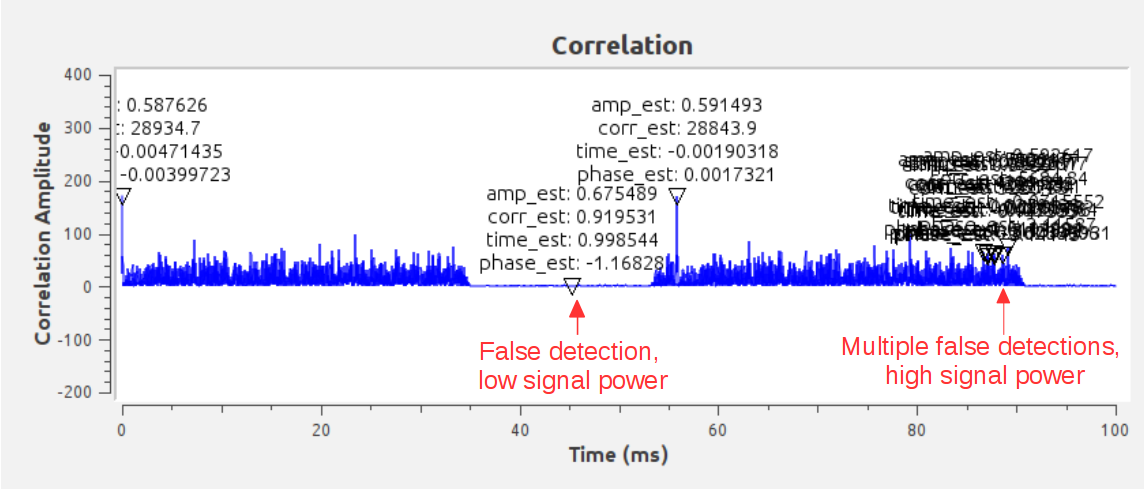
\includegraphics[width=0.8\textwidth]{img_commchain/corr_est_false2.png}
    \caption{Correlation Estimator false detections}
    \label{fig:corr_est_false2}
\end{figure}




\paragraph*{Internal working of the existing implementation }

In order to detect a correlation peak, the incoming signal is correlated with the modulated reference preamble. The squared magnitude of each correlation sample is calculated and if the squared correlation magnitude of a sample is larger than the \textit{detection threshold}, the sample is marked with a tag. Since the correlation magnitude depends on the incoming signal level, adaptive gain control should be used to normalize the signal power.\medskip

The detection method can be expressed in formulas as follows. \textit{Incoming\_signal} is the incoming symbol sequence of length $N$ and \textit{mod\_preamble} is the modulated preamble symbol sequence. The exact way to determine the \textit{detection\_threshold} is explained in the next paragraph.  

\setlength{\abovedisplayskip}{1pt}
\setlength{\belowdisplayskip}{1pt}
\begin{align*}
 corr = correlate(incoming\_signal, mod\_preamble)
\end{align*}
\begin{align*}
 corr\_mag\_sq[i] = corr[i]^2 \quad \forall i = 0\ to\ N-1
\end{align*}
\begin{align*}
detection[i] = corr\_mag\_sq[i] > detection\_threshold \quad \forall  i = 0\ to\ N-1
\end{align*}
\smallskip

Up to GNU Radio 3.7.9, the Correlation Estimator block used a fixed detection threshold. The \textit{detection\_threshold} value is relative to the power of the discrete autocorrelation of the modulated reference preamble.  The value is constant and does not depend on the incoming signal. The parameter $threshold$ can be defined by the user:

\begin{align*}
preamble\_autocorr =  \sum_{i}{|mod\_preamble[i] * mod\_preamble[i]^*|}
\end{align*}
\begin{align*}
detection\_threshold = threshold * preamble\_autocorr^2;
\end{align*}
\smallskip




In GNU Radio 3.7.10, the fixed detection threshold was changed to an adaptive threshold, to avoid the need for adaptive gain control. That implementation uses a constant false alarm rate (CFAR) detection method. The given \textit{threshold} parameter is converted to a probability of false alarm (pfa):

\begin{align*}
 d\_pfa = -\log (1- threshold)
\end{align*}
\smallskip

The final detection level is a multiplication of the average correlation magnitude of surrounding samples and the probability of false alarm:

\begin{align*}
 detection\_threshold = 4 * d\_pfa * mean(corr\_mag\_sq\ of\ surrounding\ samples)
\end{align*}
\smallskip

The decision algorithm is also slightly modified. A sample is indicated as a packet start if the sum of the squared correlation magnitude of this sample \textit{i} and the next sample \textit{i+1} is greater than the detection threshold. The sum is introduced to counter the effect of a time offset, which can spread the correlation peak over two samples.

\begin{align*}
	detection = (corr\_mag[i] + corr\_mag[i+1]) > detection\_threshold
\end{align*}
\smallskip


\subsubsection{Improved Correlation Estimator}
We modified the Correlation Estimator, and included a new block called Correlation Estimator 2 in the \textit{packetizer} module. This new block solves the problems described in the previous section, by doing several modifications in the C++ code.

\paragraph*{Solving problem 1: Increasing the maximum threshold}

The internal representation of the $threshold$ parameter variable is a float. The limited precision of a float causes numerical problems when calculating \( d\_pfa = -\log (1- threshold)\). In fact, the closest float to 1 is 0.999999880791. Anything closer to 1 will be rounded to 1 and that gives the logarithm of 0, which is impossible to compute. \medskip

By changing the internal threshold representation from float to double, a much larger threshold can be chosen.

\paragraph*{Solving problem 2: False detections when no signal}
Detecting a packet when the incoming signal level is very low is not useful, since the SNR will probably be too low to decode the packet. By adding a fixed threshold in parallel to the adaptive threshold, a minimum signal power can be set. The fixed threshold is implemented in the same way as the one in Correlation Estimator block in GNU Radio 3.7.9, by setting the minimum ratio between the correlation magnitude and autocorrelation value of the preamble.

\paragraph*{Solving problem 3: False detections at the end of the packet}

The adaptive threshold sets the detection threshold based on the mean squared magnitude of surrounding samples. The Correlation Estimator block averages all the samples that are currently being processed in the block. The amount of samples that is passed between blocks in the dataflow graph is chosen by the GNU Radio scheduler, and can change during execution.  %TODO
\reff{corr_dataflow} visualizes  which samples were considered when averaging the correlation values at a particular instant. The \textit{START} tag indicates the first sample of a dataflow sample group, and all subsequent samples up to the next \textit{START} tag are processed at once in the block.\medskip

It is clear that this way is not optimal when only a part of the sample group has a significant amplitude. In that case, the threshold will be low and false positives occur on the few samples with significant amplitude.\medskip

The problem can be solved by defining a fixed number of samples to average. In the improved implementation of the Correlation Estimator block, the amount of samples is based on the amount of samples of the modulated reference preamble. For a BPSK preamble of 64 symbols shaped with 4 symbols per sample, the Correlation Estimator will average $256/2$ samples to set the detection threshold. These samples are chosen around the sample of interest, i.e. the sample that is currently being checked.\medskip

\begin{figure}[H]
    \centering
    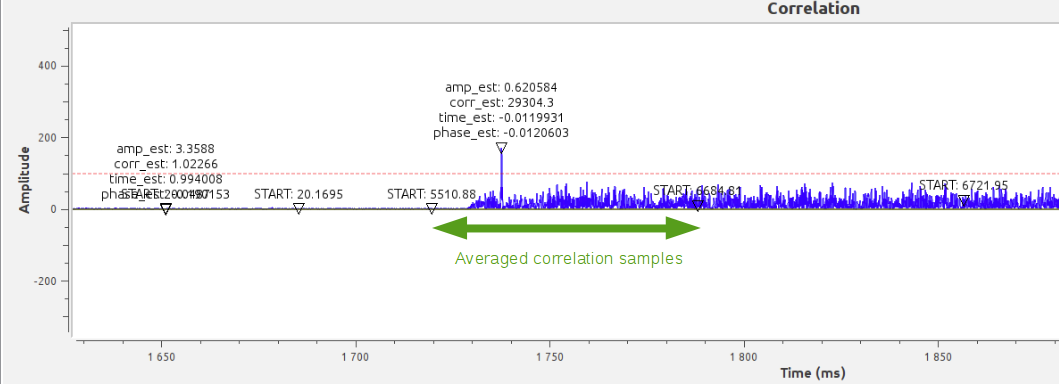
\includegraphics[width=1\textwidth]{img_commchain/corr_dataflow.png}
    \caption{{Correlation samples}}
    \label{fig:corr_dataflow}
\end{figure}

\paragraph*{Block in GNU Radio Companion}
The Correlation Estimator 2 block is also included in the new $gr$-$packetizer$ package made for this project. The block is shown in \reff{corr_est_2}. The block has two extra parameters compared to the original Correlation Estimator block: \textit{Fixed threshold} and \textit{Verbose}.
\begin{tight_itemize}
\item Symbols: symbols of the modulated and pulse shaped preamble
\item Samples per Symbol: upsampling factor 
\item Tag marking delay: tag position delay (number of samples) compared to detection instant
\item Threshold: threshold value to set the \textit{probability of false alarm} variable for the adaptive threshold
\item Fixed threshold: threshold value to set the fixed threshold, which is relative to the power of the autocorrelation
\item Verbose: output a message in the console when a peak has been detected, with the peak value, the current adaptive threshold value and the fixed detection thresholds
\end{tight_itemize}


\begin{figure}[H]
    \centering
    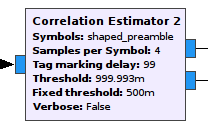
\includegraphics[width=0.35\textwidth]{img_commchain/corr_est_2.png}
    \caption{{Correlation Estimator 2}}
    \label{fig:corr_est_2}
\end{figure}

\subsection{Time and phase synchronization} \label{section_time_phase_sync}
The Correlation Estimator can derive time and phase information by looking at the correlation result. The block will communicate this information by adding the tags \textit{phase\_est} and \textit{time\_est} to the stream.\medskip

The Polyphase Clock Sync block is a time synchronizer that is compatible with the \textit{time\_est} tag. Its purpose is to realign and downsample the incoming stream so the signal samples of the output signal are sampled at exactly the peak of the sinc shape introduced by the root raised cosine filter. The block immediately applies the matched pulse shaping filter using a polyphase filter bank, so the block outputs constellations symbols.\medskip

Costas Loop is a phase synchronizer that optionally uses the \textit{phase\_est} tag. In fact, Costas Loop uses a phase-locked loop to track the carrier frequency. \reff{costas_phase} shows the effect of Costas Loop when a fixed phase offset is seen by the receiver. \reff{costas_freq} illustrates the case where a carrier frequency offset has been applied. Costas Loop will lock to the carrier frequency and align constellations to their correct positions. The \textit{phase\_est} tag helps to quickly correct the phase by indicating the estimated phase offset.\medskip

GNU Radio's Costas Loop expects the modulation order as an input parameter. The modulation order for phase-shift keying modulations is \(2^{N}\), where $N$ is the number of bits per symbol. Costas Loop in GNU Radio is limited to the modulation orders 2 (\gls{bpsk}), 4 (\gls{qpsk}) and 8 (\gls{8psk}). \medskip

The packet encoder/decoder pair implemented in this project supports different constellation types for preamble, header and payload. This implies that the Costas Loop block can only be applied after the header and payload have been split by the Preamble/Header/Payload Demux block. The header decoder stream and payload decoder stream have their own phase synchronizers that receive bursts of header or payload data, as shown in \reff{packet_decoder_grc}. The phase can have large discontinuities between those bursts, which makes it more difficult for the phase-locked loop to lock to the carrier and reduces the performance of Costas Loop. \medskip


\begin{figure}[H]
    \centering
    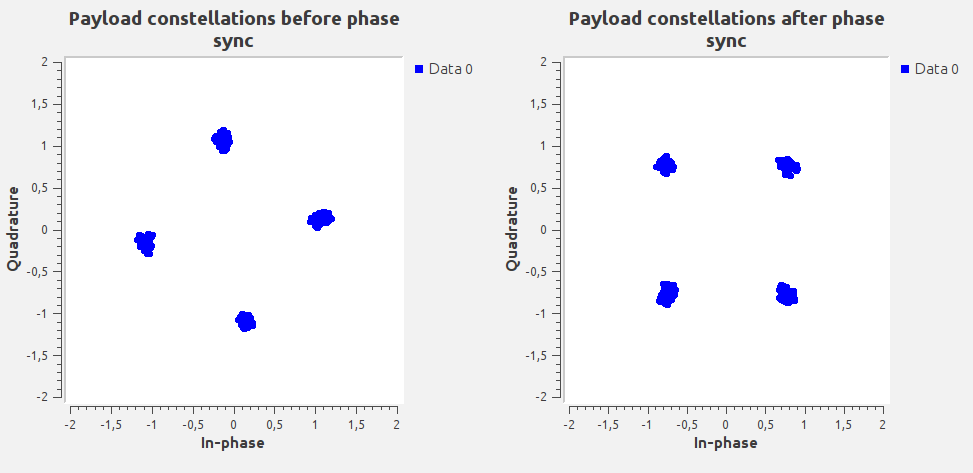
\includegraphics[width=0.8\textwidth]{img_commchain/phase_sync.png}
    \caption{Effect of Costas Loop when receiving constellations with a fixed phase offset }
    \label{fig:costas_phase}
\end{figure}



\begin{figure}[H]
    \centering
    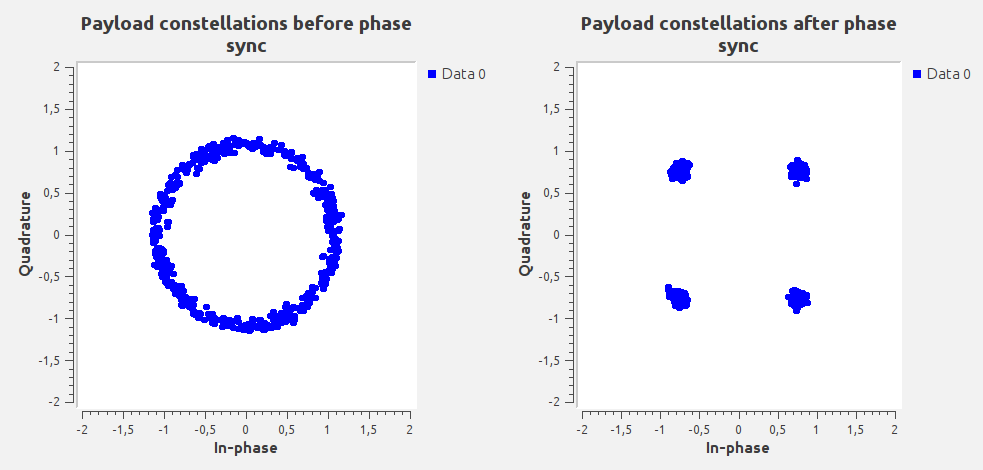
\includegraphics[width=0.8\textwidth]{img_commchain/phase_sync2.png}
    \caption{Effect of Costas Loop as a frequency tracker}
    \label{fig:costas_freq}
\end{figure}

\subsubsection{Test systems}
\textit{test\_time\_phase\_sync.grc} is an extension of mapping example \textit{test\_mapping.grc}. The symbols are shaped with a root raised cosine filter. A channel model is added to simulate a time offset, frequency offset, phase offset and noise in the signal. Time and phase synchronization is added with the Polyphase Clock Sync block and Costas Loop. A BER output is also provided, which can be used to analyze the effects of the channel. It is used to verify the correct working of the communication chain.





\subsection{Data whitening}

Data grouped in packets can contain long sequences of 0's and 1's. The lack of signal variation can be problematic for adaptive circuits such as adaptive gain control and phase-locked loops.\medskip

Data whitening or scrambling is a technique to eliminate long sequences of 0's and 1's. A simple additive synchronous whitener is implemented in this project, which whitens incoming data bytes by applying $XOR$ operations with a pseudo-random sequence. Data can be dewhitened by applying the same $XOR$ operations. The implementation is synchronous because the pseudo-random sequence needs to be reset to align with the data stream. Since this project uses packet-based communications, synchronization is straightforward: at the start of a packet, the random sequence is reset.\medskip

The whitener implementation is split in a kernel and a block interface. The kernel is a general implementation which can be used as a standalone whitener. The packet encoder uses this kernel to whiten incoming data. The kernel is in fact both a whitener and dewhitener, since the inverse operation of an $XOR$ is itself.\medskip

The block interface wraps the kernel in a standalone GNU Radio block. It manages the input and output of items and provides an interface to configure the block. The whitener block then initializes the whitener kernel depending on the given arguments.

\subsubsection{Whitener kernel}
The whitener kernel is a C++ class that performs the whitening operations. The class $gr/packetizer/kernel/whitener.h$ defines three constructors:
\begin{enumerate}
\item $whitener();$\\
Initializes a whitener object for 8 significant bits per byte using a linear-feedback shift register.

\item $whitener(int\ bits\_per\_byte);$\\
Initializes a whitener object for $bits\_per\_byte$ significant bits per byte using a linear-feedback shift register.

\item $whitener(std::vector<unsigned\ char> random\_mask, int\ bits\_per\_byte);$\\
Initializes a whitener object for $bits\_per\_byte$ significant bits per byte using the given $random\_mask$ to XOR data with. If $random\_mask$ is an empty vector, a pre-computed random mask will be used.
\end{enumerate}

After initialization, the whitener object can be used to process data by executing its method:

\begin{minted}[frame=single,breaklines=true]{C}
/*!
* Do the whitening. Starts reading data in at pointer data_in
* Starts outputting data at data_out
* Processes data_length bytes of data.
*/
void
do_whitening(const unsigned char* data_in, unsigned char* data_out, unsigned int data_length, unsigned int whitening_offset);
\end{minted}

\subsubsection{Whitener block}

The whitener block is called the Tagged Stream Whitener. A \textit{tagged stream} in GNU Radio expects a stream where data is combined in packets with a tag indicating the packet start and length. The block is both a whitener and dewhitener. After whitening, the original data can be recovered by applying the same block with the same parameters on the whitened stream.

\begin{figure}[H]
    \centering
    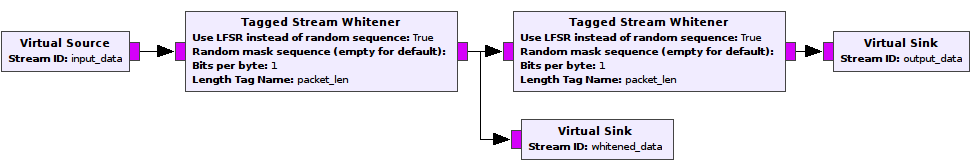
\includegraphics[width=1\textwidth]{img_commchain/whitener_chain.png}
    \caption{The Tagged Stream Whitener in GNU Radio Companion. The left block whitens the data and the right one dewhitens data.}
    \label{fig:whitener_data}
\end{figure}


\subsubsection{Test system}
\textit{test\_whitener.grc} illustrates the use of the \textit{Tagged Stream Whitener} blocks.



\begin{figure}[H]
    \centering
    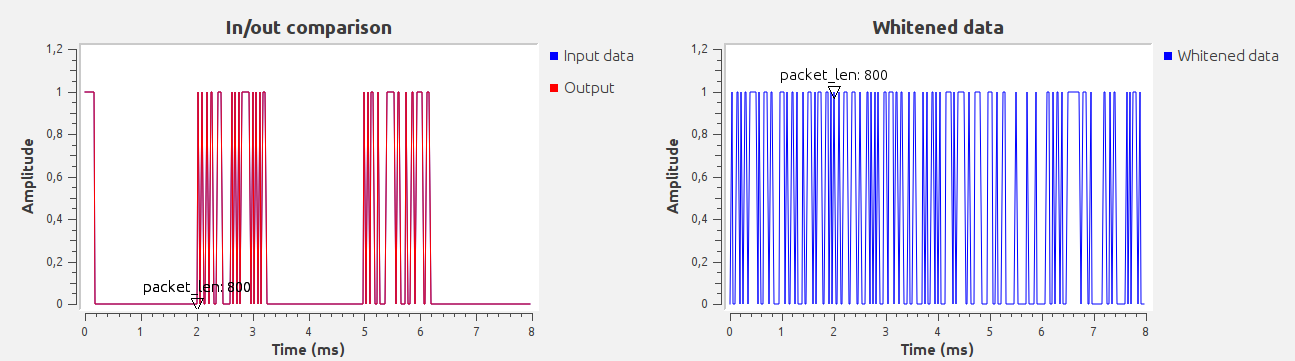
\includegraphics[width=1\textwidth]{img_commchain/whitener.png}
    \caption{Non-whitened data on the left has long sequences of 0 bits. }
    \label{fig:whitener_data}
\end{figure}

\begin{figure}[H]
    \centering
    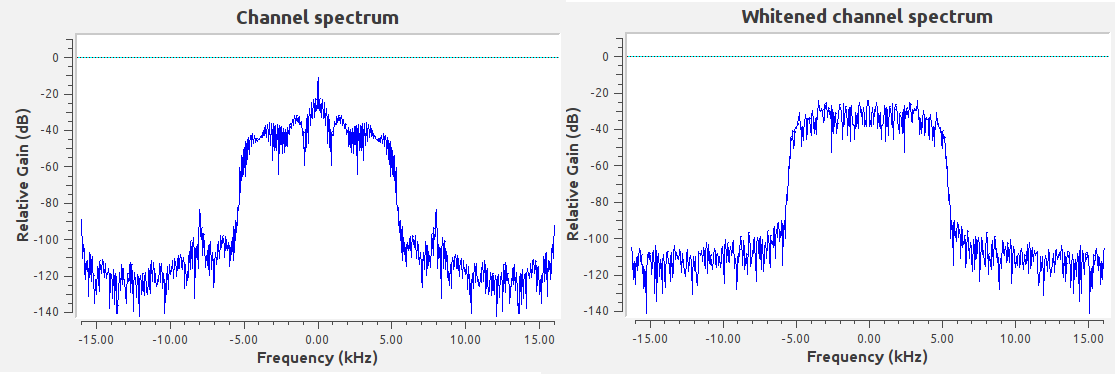
\includegraphics[width=1\textwidth]{img_commchain/whitened_spectrum.png}
    \caption{The non-whitened spectrum is unbalanced and has a DC peak. }
    \label{fig:whitener_spectrum}
\end{figure}




\subsection{Forward Error Correction}

\gls{fec} or channel coding pre-processes the data by adding redundancy to make communications more reliable in noisy channels. Encoding data in a redundant way is done with an error-correcting code.  \medskip

GNU Radio has a dedicated package with \gls{fec} modules called $gr$-$fec$ which is extensively documented. \cite{gr_fec_docs} % REF https://gnuradio.org/doc/doxygen/page_fec.html
The \gls{fec} API is split on two levels: variables and deployments. A variable implements error-correcting code in encoding and decoding methods. A deployment is the connection between the flowgraph and the variable. It will handle the setup and data passing between blocks. \medskip

Several error-correcting codes are defined. A standard convolutional coder is used in this project in combination with the FEC Extended Tagged Encoder and FEC Extended Tagged Decoder as deployments. The \gls{fec} encoder is placed right before the packet encoder, and the \gls{fec} decoder right after the packet decoder. The FEC Extended Tagged Decoder has a float input and can use soft-decision decoding. 



\subsubsection{Test systems}
\textit{test\_fec.grc} illustrates the use of the \textit{FEC Extended Tagged Encoder} and \textit{FEC Extended Tagged Decoder}. Note that the FEC encoder expects a data stream of bytes with 1 significant bit per byte. The output of the encoder is manually mapped to soft bits (-1 and 1). A separate CC Decoder object is set for each FEC decoder.\medskip

\textit{encdec\_custom\_fec.grc} implements a packet encoder and decoder combined with forward error correction,  with hard and soft decisions.



\subsection{Communication chain example systems}
\subsubsection*{Communication chain with Extended Packet Encoder/Decoder blocks}
\textit{chain\_custom.grc} implements the full communication chain with packet encoder, pulse shaper, channel modeler, adaptive gain control, correlation estimator (preamble detector), time synchronization and the packet decoder (which includes phase synchronization).

\subsubsection*{Communication chain with RX receiver built with fundamental blocks}
\textit{chain\_rx\_debug.grc} implements the same communication chain as the previous example. In this example, the packet decoder is built using separate blocks, in order to debug the individual components of the packet decoder. This example can also be used to implement extensions of the packet decoder.

\subsubsection*{Communication chain with RX receiver built with fundamental blocks}
\textit{chain\_rx\_debug\_differential.grc} is the same as \textit{chain\_rx\_debug.grc}, but with differential decoding.

